\chapter{Caracteristicas de transferencia del JFET}
  En el análisis de los transistores de efecto de campo de juntura (JFET), resulta fundamental comprender la relación
  entre la tensión aplicada entre compuerta y fuente (\(V_{GS}\)) y la corriente de drenaje (\(I_D\)). Esta relación se
  conoce como característica de transferencia, ya que describe cómo la señal de entrada (voltaje de control)
  regula la corriente de salida del dispositivo.  

  La dependencia entre estas magnitudes está dada por la ecuación de Shockley, la cual permite predecir el
  comportamiento del JFET en la región de saturación. A partir de esta ecuación es posible determinar cómo varía \(I_D\)
  en función de \(V_{GS}\), estableciendo un modelo matemático que refleja el efecto de la compuerta sobre la conducción
  del canal:  

  \begin{equation}
    I_D = I_{DSS} \left( 1 - \frac{V_{GS}}{V_p} \right)^2
  \end{equation}
  
  A partir de los datos experimentales obtenidos en la curva de salida \(I_D(V_{DS})\), es posible determinar los
  valores de \(I_{DSS}\) y de la tensión de pinch-off \(V_p\). Con estos parámetros, se puede trazar la ecuación de
  Shockley y representar la característica de transferencia del JFET.  
  
  \begin{figure}[!ht]
    \centering
    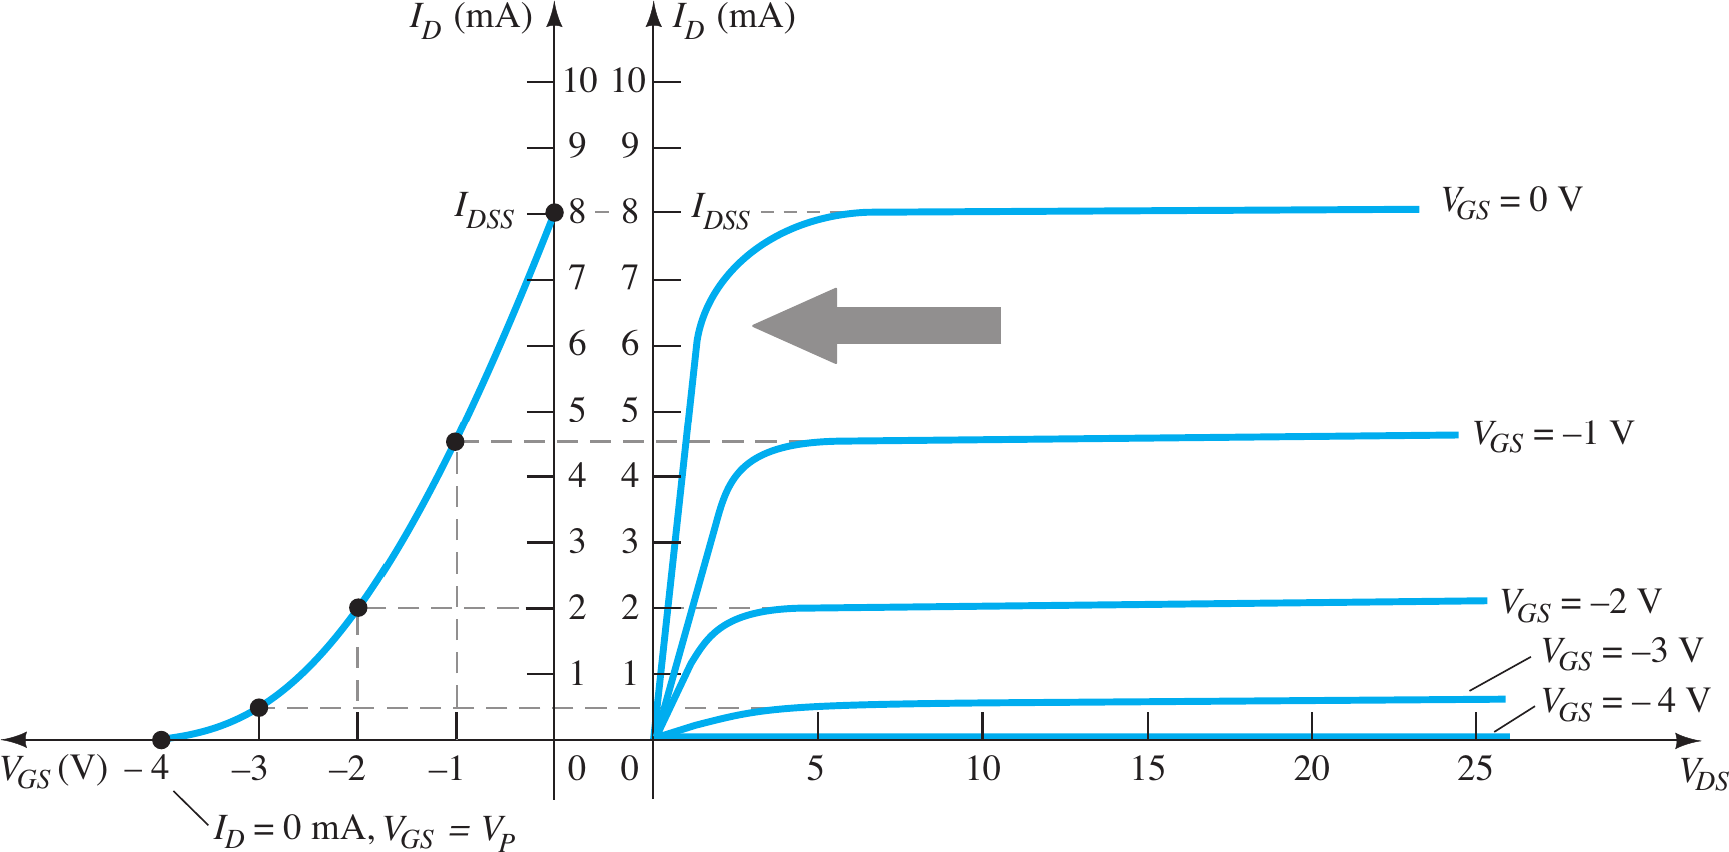
\includegraphics[width=1\textwidth]{images/grafico_transferencia.png}
    \caption{característica de transferencia del JFET obtenida a partir de la ecuación de Shockley.}
    \label{fig:transferencia}
  \end{figure}

\section{Actividad de Simulación}
    Se propuso implementar el circuito de la figura \ref{crkt:jfet-transf} en el simulador LTSpice, y hacer que la fuente
    $V1$ varíe desde $0V$ a $8V$ en pasos de $0.1V$, y por cada variacion de la fuente $V1$, que la fuente $V2$ varie de
    $0V$ a $15V$ en pasos de $0.1V$ para poder recrear una familia de curvas que expongan el comportamiento de la
    corriente $I_D$ en función del voltaje drain-source $V_{DS}$ por cada $V_{GS}$.
    \begin{figure}[!ht]
      \centering
      \begin{minipage}{0.45\textwidth}
        \begin{tikzpicture}
          % Paths, nodes and wires:
          \node[njfet](N1) at (2.25, 2.73){} node[anchor=west] at (N1.text){$BF245B$};
          \draw (4.75, 3.48) to[battery, l={$V2$}] (4.75, 1.98);
          \draw (4.75, 3.46) -- (4.75, 5.21) |- (2.25, 5.21) -| (2.25, 3.48);
          \draw (2.25, 1.96) -- (2.25, 0.73);
          \draw (4.75, 1.98) -- (4.75, 0.73);
          \node[ground] at (0.25, 0.73){};
          \node[ground] at (2.25, 0.73){};
          \node[ground] at (4.75, 0.73){};
          \draw (0.25, 1.25) to[battery, l={$V1$}] (0.25, 2);
          \draw (1.27, 2.46) -| (0.25, 2);
          \draw (0.25, 0.73) -| (0.25, 1.25);
        \end{tikzpicture}
        \caption{circuito de prueba para caracteristicas de trasnferencia.}
        \label{crkt:jfet-transf}
      \end{minipage}
      \hfill
      \begin{minipage}{0.45\textwidth}
        \begin{lstlisting}[style=ltspice, caption={Parámetros de simulación LTspice}, label=list:jfet-transf]
.MODEL  BF245B   NJF VTO = -2.3085E+000 BETA = 1.09045E-003 LAMBDA = 2.31754E-003 RD = 7.77648E+000 RS = 7.77648E+000 IS = 2.59121E-016 CGS  = 2.00000E-012 CGD  = 2.20000E-012 PB = 9.91494E-001 FC = 5.00000E-001
.dc V2 0 15 .1 V1 0 8 .1
        \end{lstlisting}
      \end{minipage}
    \end{figure}
    \begin{figure}[!ht]
      \centering
      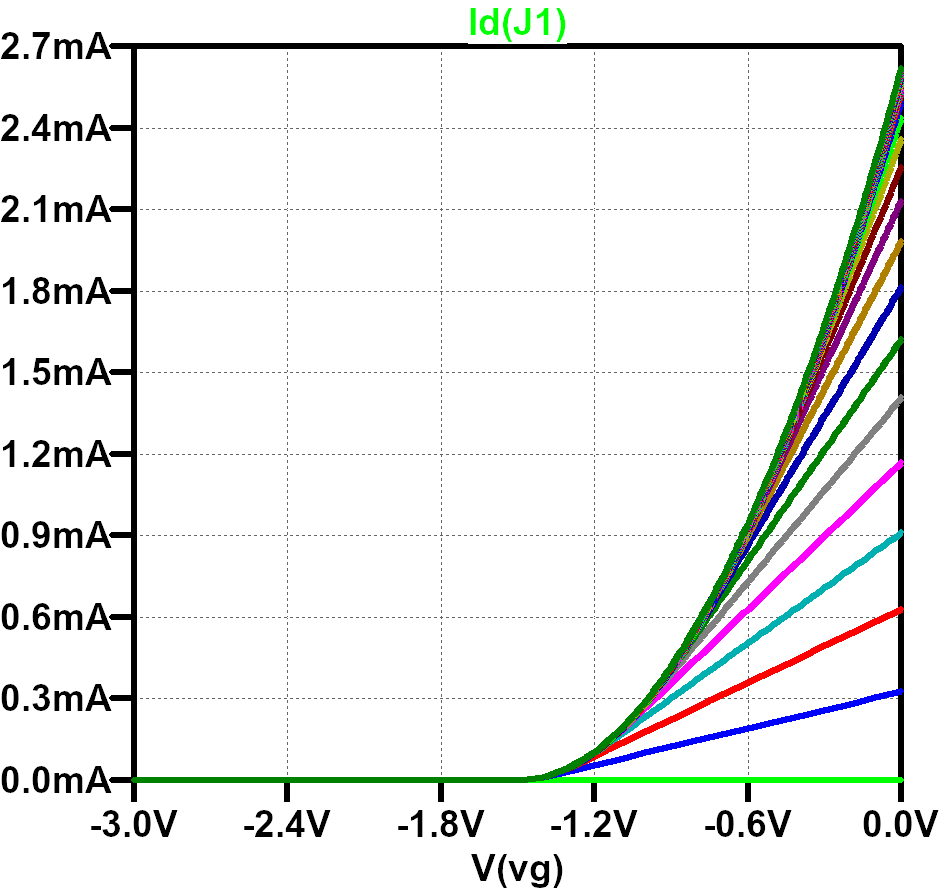
\includegraphics[width=0.8\textwidth]{images/transferencia-id_vds-vgs.png}
      \caption{resultados de simulación para caracteristicas de transferencia del JFET.}
      \label{fig:sim.transf}
    \end{figure}

    Para poder apreciar mejor los resultados de la figura \ref{fig:sim.transf}, se redujo el barrido de la fuente $V1$
    hasta $3V$ en pasos de $0.2V$. Como se puede ver, el modelo describe perfectamente la famila de curvas de
    $I_{D_{(V_{DS}, \, V_{GS}})}$. La unica diferencia observable comparada con la grafica presentada por el fabricante es el
    valor de $I_{DSS}$.
